\documentclass[a4paper]{scrartcl}

\usepackage[
typ={ib},
fach=Informatik,
farbig,
%module={ohne}
]{schule}
\hypersetup{hidelinks}

\usepackage{fontspec}
\usepackage{fourier-otf}

\usepackage[scale = 0.1]{jetbrainsmono-otf}

\setmonofont[Scale = MatchLowercase]{jetbrainsmono-light}

\usepackage{scrlayer-scrpage}
\ifoot{
	
	
\includegraphics[width=0.35\linewidth]{GHSE-Logo}
	
}

\usepackage[ngerman]{babel} 

\usepackage{shellesc}
\usepackage{minted}
\usepackage[]{float}
\usepackage{microtype}	


\date{}

\title{Konkrete Werte in Sequenzdiagrammen}
\begin{document}




\section*{Konkrete Werte in Sequenzdiagrammen angeben}


Im folgenden Codebeispiel werden die Klasse \texttt{Student} und die Methode \texttt{getGreeting} definiert.

\begin{minted}{java}
record Student(String name, int age) {
	
    public String getGreeting() {
        return "Hello, my name is " + name + ", I am " + age + " years old"
    }
    
}
\end{minted}

Wenn aus dem Zusammenhang klar ist, wie der Rückgabewert eines Methodenaufrufs lautet, 
kann auch ein konkreter Wert in das Sequenzdiagramm eingetragen werden.
\begin{figure}[H]
    \centering
    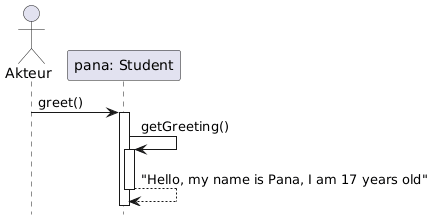
\includegraphics[width=\linewidth]{pana}
    \label{fig:s2}
\end{figure}
Genauso können bekannte Parameter direkt im Sequenzdiagramm angegeben werden.

\end{document}
